%\begin{itemize}
%    \item
%        Weshalb wurde das benutzte mathematische Modell gew\"ahlt?
%    \item
%        Weshalb wird ein Schaltregler benutzt?
%    \item
%        Weshalb wurde ein eigenes PCB entwickelt statt ein Steckbrett verwendet?
%    \item
%        Wie soll unser Ger\"at bedient werden k\"onnen?
%\end{itemize}

Underpinning our device  is a microcontroller which is primarily responsible for
handling I/O tasks (such  as  user  interaction and the display) and controlling
the step-down converter. Power  delivery  is  realised  with a prebuilt DC power
supply unit.

With an eye towards  potential serial production, we developed our own PCB. This
allows  tight  control  over impedances  in  the  connections  between  critical
components and brings the behavior of the prototype device much closer to a mass
produced version than a breadboard solution could. This is because trace routing
lengths and component placement are  crucial factors, as is discussed in section
\ref{sec:verification}  (p.  \pageref{sec:verification}ff), \emph{Verification}.

Users can  interact with our device  either through a push-twist  button and a
display on the device itself or from  a PC connected by USB using our software
\emph{Smooth} (section \ref{subsec:frontend}, p. \pageref{subsec:frontend}ff).


% **************************************************************************** %
\subsection{Concept of Regulation Circuit}
% **************************************************************************** %

\begin{minipage}{0.5\textwidth}
    \center
    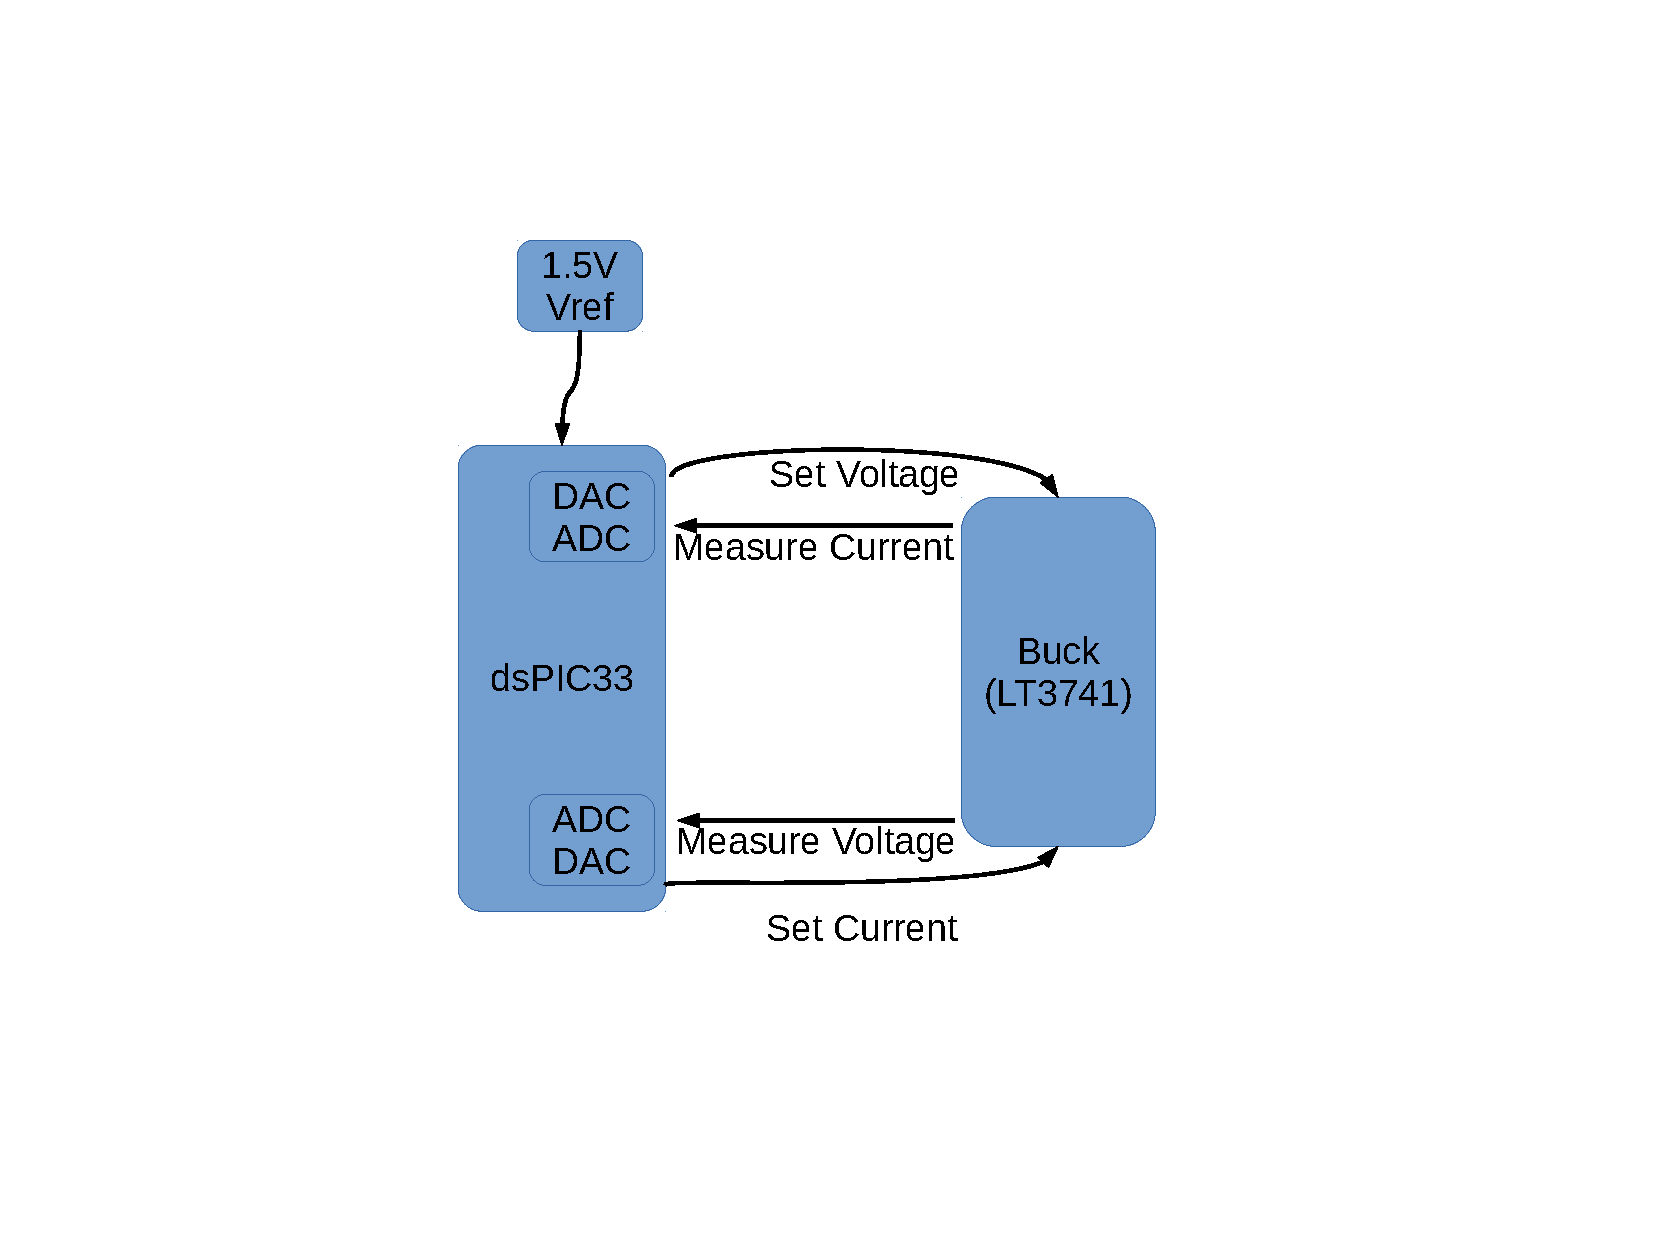
\includegraphics[width=\textwidth,trim=140 140 120 100,clip]{images/block-diag-control.pdf}
    \captionof{figure}{Block diagram of control circuit}
    \label{fig:controlcircuit:schcematic}
\end{minipage}
\begin{minipage}{0.5\textwidth}
    \center
    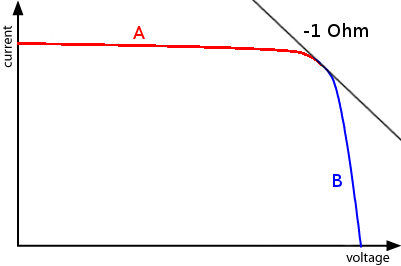
\includegraphics[width=\textwidth]{images/vi-curve.png}
    \captionof{figure}{IV-Curve with \SI{-45}{\degree} slope indicated}
    \label{fig:controlcircuit:vicurve}
\end{minipage}

Emulation of the IV characteristic  curve  is  achieved  accurately by measuring
both output voltage and output current. If  the  operating  point  is  above the
\SI{-45}{\degree} slope (``A'' in  figure \ref{fig:controlcircuit:vicurve}) then
it is more accurate  to  operate  the  regulator  in  constant  current mode. In
contrast, if the operating point is below  the \SI{-45}{\degree} slope (``B'' in
figure \ref{fig:controlcircuit:vicurve}) then it is more accurate to operate the
regulator in constant voltage mode. A more detailed explanation can  be found in
section         \ref{subsec:finding-the-operating-point}         on         page
\pageref{subsec:finding-the-operating-point}.


\subsection{Goals of the model}

The aim  was  to  find  the sweet spot between usability and accuracy. Our model
should  have  a  small,  comprehensive  set  of parameters which can  be  easily
understood by the user. This includes solar irradiation, as we want to model how
clouded skies or a partially covered module affects its output.


\subsection{Model for one solar cell}

The single diode model of the ideal PV cell\cite{ref:villa:pvmodel} servers as a
basis for our model.  The  IV characteristic of this model can be expressed with
\begin{equation} \label{eq:IV_old}
    I = I_{pv} - I_o \left[ \exp \left( \frac{V}{V_T} \right) - 1 \right]
\end{equation}
where $I_{pv}$ is the generated current, $I_o$ is the diode current and $V_T$ is
the thermal  voltage.  Although  these  three  parameters depend on the junction
temperature,  the  inclusion  of  the junction temperature into our model  as  a
parameter would only contribute a minor correction factor,  negligible  for  our
purposes.  For  this  reason  we  can simplify our model if we assume  that  the
temperature is equal to  the  nominal  temperature  $T_n = 298.15K$. The thermal
voltage is defined as
\begin{equation}
    V_T = a k T / q
\end{equation}
where  $T$ is the junction temperature, $k$ is the Boltzman-constant, $q$ is the
elementary  charge  and  $a$  is the diode ideality factor, which typically lies
around 1.2 for silicon substrates. This gives us $V_T \approx  30.8mV$  for  one
cell. The current generated by the cell is defined as
\begin{equation}
    I_{pv} = \left( I_n + K_I \Delta_T \right) \frac{G}{G_n}
\end{equation}
where $I_n$ is the  nominal  current and $G$ and $G_n$ is the actual and nominal
solar   irradiation,   respectively.    A    common    optimisation,   according
to\cite{ref:villa:pvmodel}, is to set $I_n \approx I_{sc}$ and again assume that
the  temperature  is  constant  ($T  =  T_n$), giving  us  $\Delta_T  =  0$  and
simplifying this formula to
\begin{equation} \label{eq:I_pv}
    I_{pv} = I_{sc} \frac{G}{G_n}
\end{equation}
Finally, the  diode  leakage  current  at  the nominal temperature \footnote{For
other temperatures please see \cite{ref:villa:pvmodel}} is
\begin{equation} \label{eq:I_o}
    I_o = \frac{I_{sc}}{e^{V_{oc} / V_T} - 1}
\end{equation}
If  we   insert   equations   \eqref{eq:I_o}   and   \eqref{eq:I_pv}  back  into
\eqref{eq:IV_old} we yield
\begin{equation}
    I = I_{sc} \left( \frac{G}{G_n} - \frac{e^{\frac{V}{V_T}}-1}{e^{\frac{V_{oc}}{V_T}}-1} \right)
\end{equation}
If we now assume $V_{oc} > 5 * V_T$ we can  say  that  $e^{\frac{V_{oc}}{V_T}}-1
\approx e^{\frac{V_{oc}}{V_T}}$ and our final formula becomes
\begin{equation} \label{eq:IV}
    I = I_{sc} \left( \frac{G}{G_n} - e^{\frac{V - V_{oc}}{V_T}} \right)
\end{equation}


\subsection{Model for multiple Cells in Series}

If the solar irradiation is the same  for  every  cell in series, then the whole
array  can be simulated using equation \eqref{eq:IV}, where $V_{oc}$  and  $V_T$
are linearly scaled with the number of cells.

If the irradiation isn't the same for all  cells,  such  as  when  one  cell  is
shaded, a more complex model must be used.
\begin{figure}[h]
	\center
    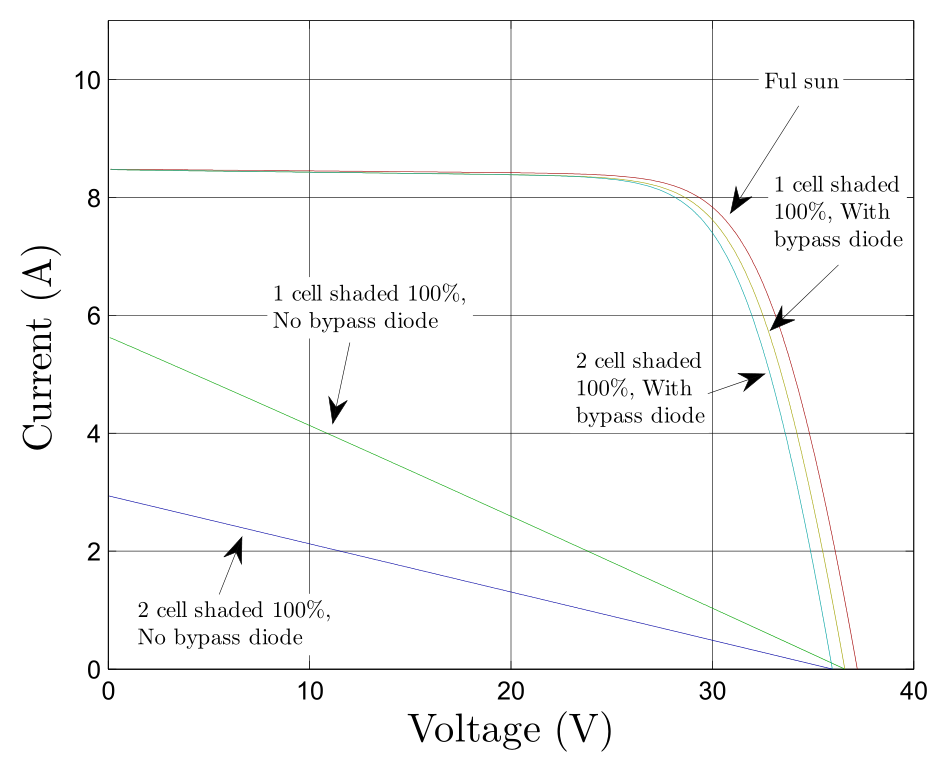
\includegraphics[width=.5\textwidth]{images/model/shaded.png}
    \caption{I-V curves for different configurations and shaded cells\cite{ref:tian:model}}
    \label{fig:model:shaded}
\end{figure}

Figure \ref{fig:model:shaded}  shows  what  varied  characteristics  of a shaded
PV-module  look  like  and  how  bypass  diodes affect them. In our model we can
imitate  the  I-V  curve of an array with a shaded cell and no bypass  diode  by
setting $V_T = V_{oc}$.

\begin{figure}[h]
	\center
    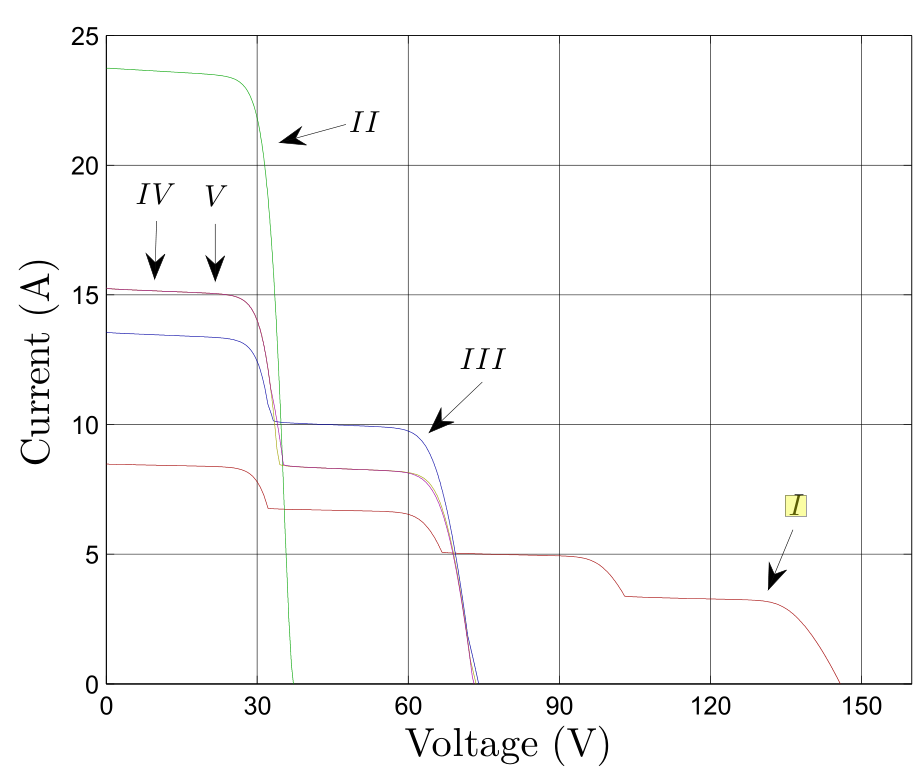
\includegraphics[width=.5\textwidth]{images/model/steps.png}
    \caption{The typical characteristic of modules connected in series or in parallel}
    \label{fig:model:steps}
\end{figure}
The  characteristic  curves  shown  in  figure  \ref{fig:model:steps}  show  how
``steps'' emerge when two or more modules  with bypass diodes, which are exposed
to different irradiation intensities, get  connected in series. To simulate this
behaviour, we take  a number of curves with decreasing short circuit current and
increasing  open  circuit  voltage  and  determine  which curve is applicable by
checking  what  curve  returns  the  maximum  current  for  the  given  voltage.

